\documentclass[xcolor=dvipsnames]{beamer}
%
% Choose how your presentation looks.
%
% For more themes, color themes and font themes, see:
% http://deic.uab.es/~iblanes/beamer_gallery/index_by_theme.html
%
\mode<presentation>
{
  \usetheme{Frankfurt}    % or try Darmstadt, Madrid, Warsaw, ...
  \usecolortheme{crane}   % or try albatross, beaver, crane, ...
  \usefonttheme{default}  % or try serif, structurebold, ...
  %\setbeamertemplate{navigation symbols}{}
  \setbeamertemplate{caption}[numbered]
} 

\usepackage[english]{babel}
\usepackage[utf8x]{inputenc}
\usepackage{wrapfig}
\usepackage{booktabs}% http://ctan.org/pkg/booktabs
\usepackage{array}% http://ctan.org/pkg/array
\newsavebox{\mybox}% Store some content in a box
\newcolumntype{G}{@{}>{\begin{lrbox}{\mybox}}l<{\end{lrbox}}@{}}% a column that Gobbles it's entries
\usepackage{adjustbox}


\usepackage[]{algorithm2e}

\usepackage{graphicx,calc}
\newlength\myheight
\newlength\mydepth
\settototalheight\myheight{Xygp}
\settodepth\mydepth{Xygp}
\setlength\fboxsep{0pt}
\newcommand*\inlinegraphics[1]{%
  \settototalheight\myheight{Xygp}%
  \settodepth\mydepth{Xygp}%
  \raisebox{-\mydepth}{\includegraphics[height=\myheight]{#1}}%
}


\title[Your Short Title]{Greedy Heuristics for Set Cover}
\author{Eirini Asteri, Jessica Hoffmann}
\institute{University of Texas, Austin}
\date{}

\begin{document}

\begin{frame}
  \titlepage
\end{frame}

% Uncomment these lines for an automatically generated outline.
\begin{frame}{Outline}
  \tableofcontents
\end{frame}

\section{Set Cover \& Greedy Algorithm}
\begin{frame}
\frametitle{Set Cover Problem \& Greedy Algorithm}
\begin{minipage}{0.45\textwidth}
\begin{overlayarea}{\textwidth}{0.5\textheight}
\only<1>{
\includegraphics[width=\columnwidth]{frame1.pdf}}% 
\only<2>{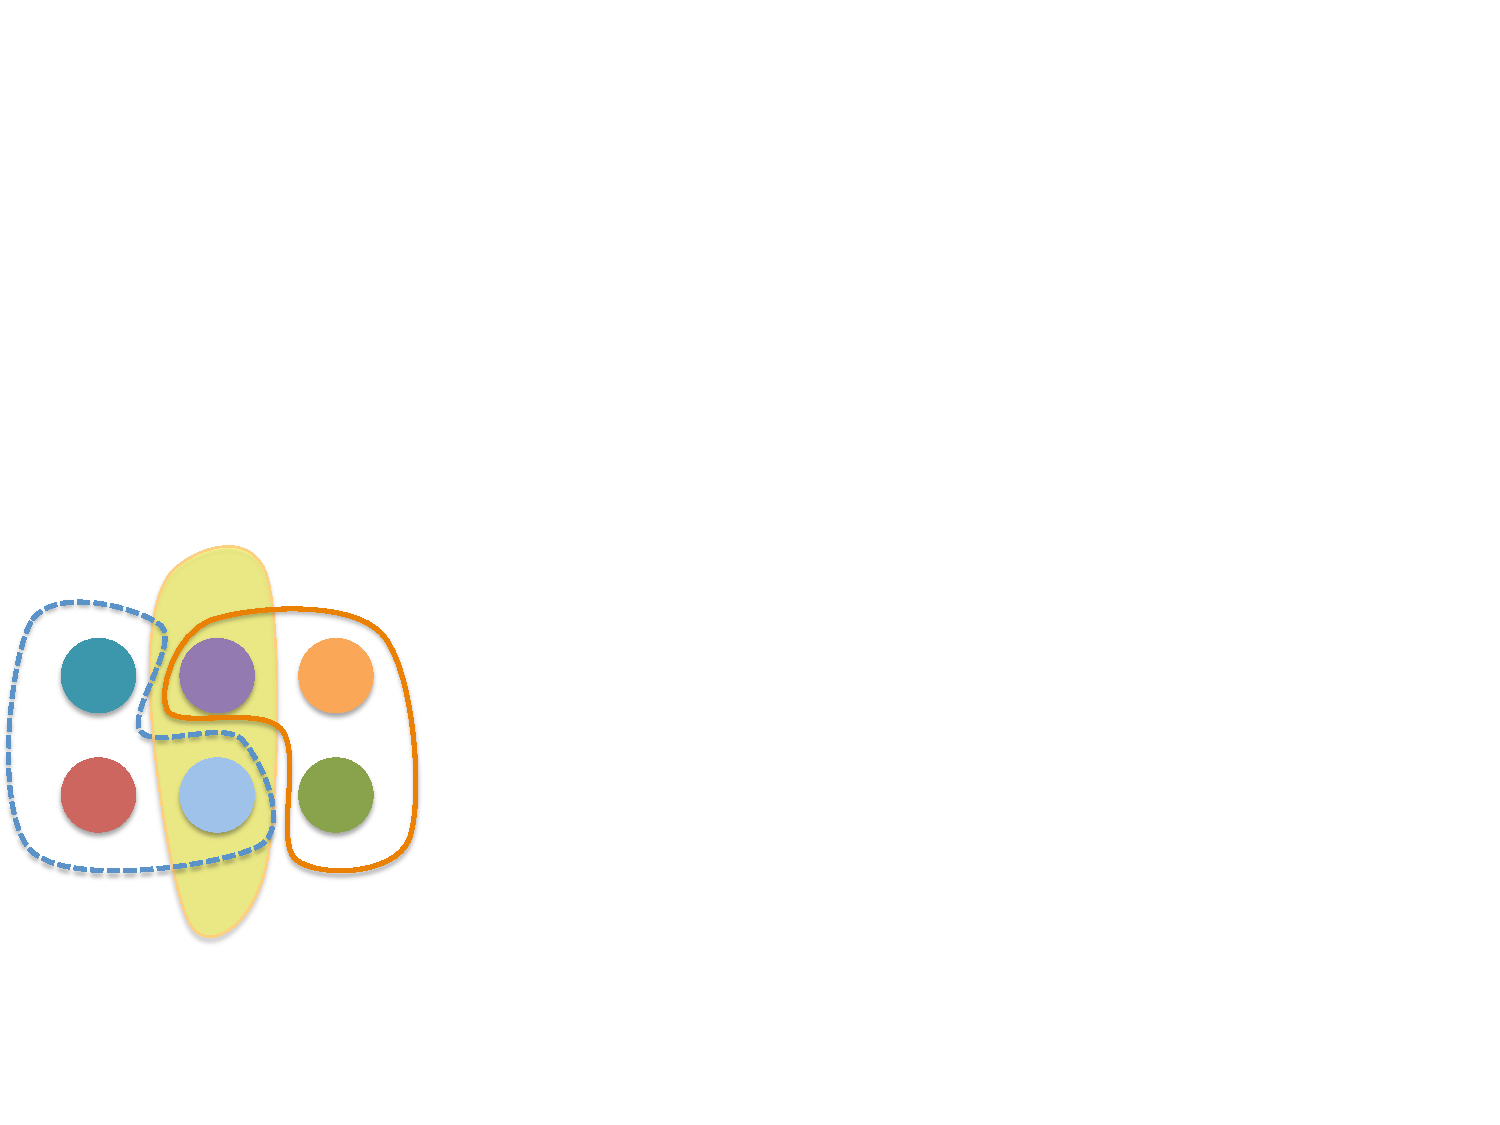
\includegraphics[width=\columnwidth]{frame2.pdf}}% 
\only<3-5>{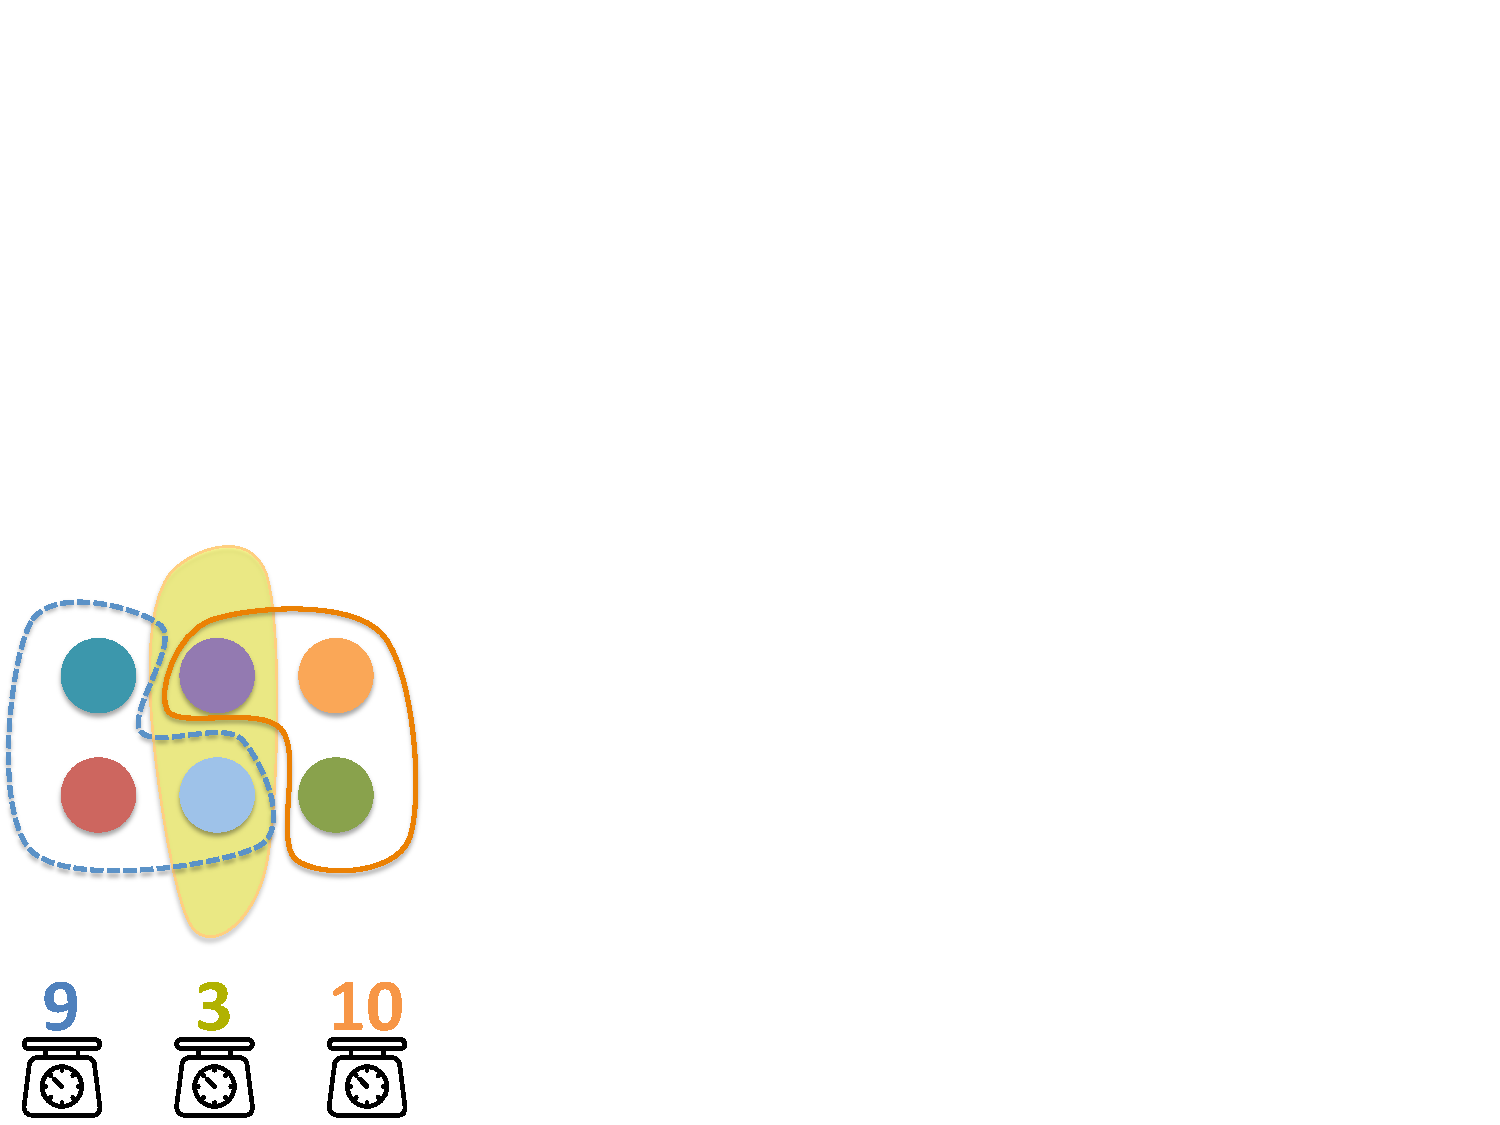
\includegraphics[width=\columnwidth]{frame3.pdf}}%
\end{overlayarea}%
\end{minipage}%
\begin{minipage}{0.55\textwidth} 
\begin{itemize}
\item<1-> Number of distinct elements $e_i$
\item<2-> Number of sets $S_j$
\item<3-> A weight for each set $w_j$
\item<4-> \textbf{Goal} Find set cover with minimum weight
\item<5> \textbf{Greedy Choice} $$best\_set = \arg \min_{l} \cfrac{w_l}{|\hat{S}_l|}$$
\end{itemize}
\end{minipage}
\end{frame}

\begin{frame}
\frametitle{Basic Preprocessing}
\begin{block}{Get rid of redundant sets \inlinegraphics{sweep.eps}}
If $S_{small} \subseteq S_{big}$ and $\text{weight}(S_{small})\geq \text{weight}(S_{big})$ then $S_{small}$ is a redundant set.
\end{block}
\end{frame}


\section{Greedy Heuristics}
\begin{frame}
\frametitle{Heuristics, Intuition}
\begin{minipage}{0.30\textwidth}
\begin{overlayarea}{\textwidth}{0.5\textheight}
\only<1-3>{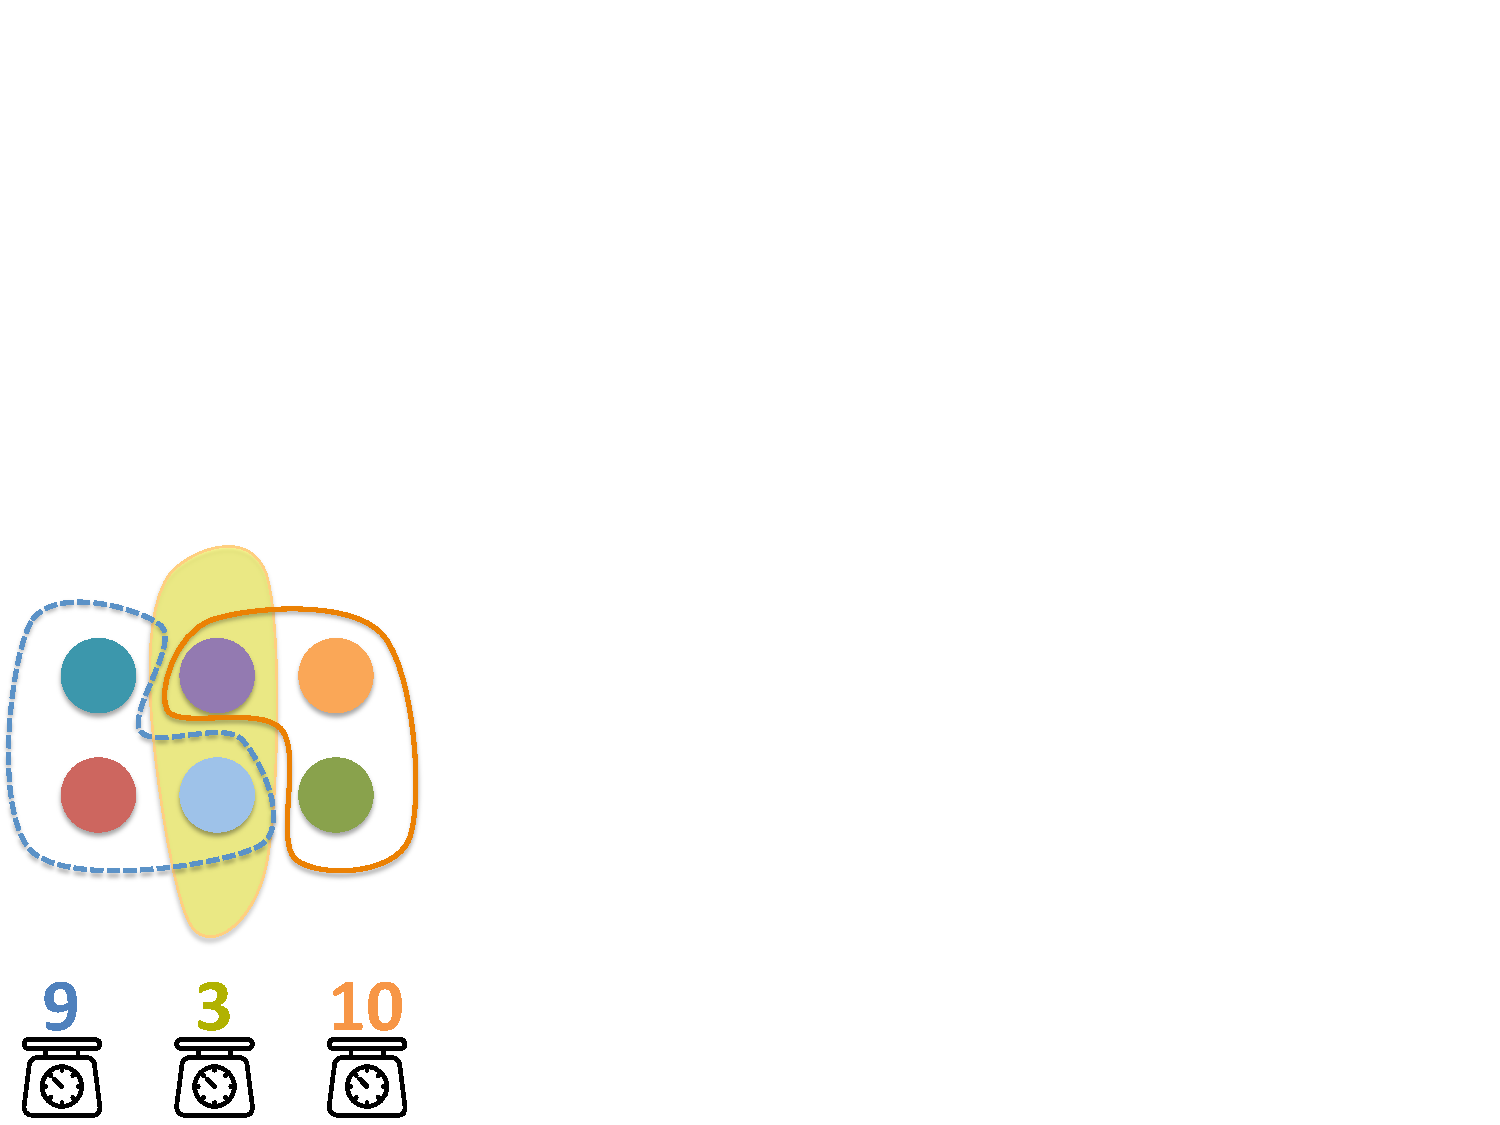
\includegraphics[width=\columnwidth]{frame3.pdf}}% 
\only<4-5>{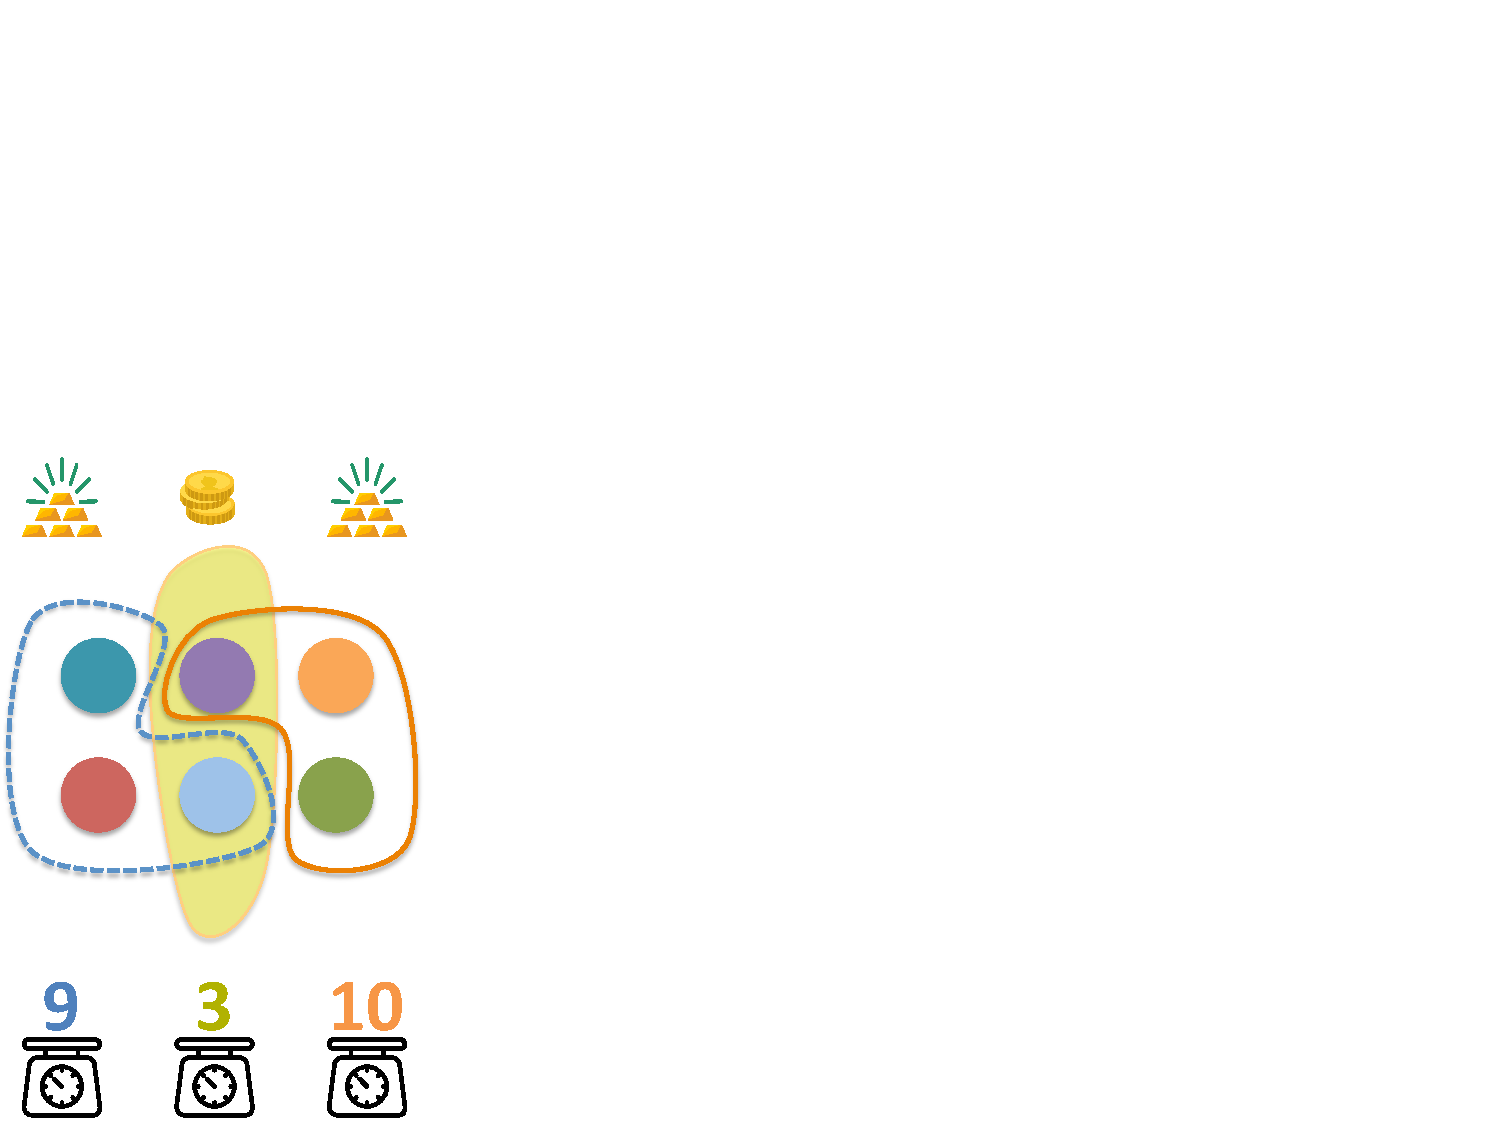
\includegraphics[width=\columnwidth]{value.pdf}\vfill}% 
\end{overlayarea}%
\end{minipage}%
\begin{minipage}{0.70\textwidth} 
\begin{itemize}
\item<1-> Elements with frequency $1$ should be covered first
\item<2-> Extend idea to \textbf{``infrequent''} elements
\item<3-> Assign a value to each element
  	$$ \text{value(element)} = \cfrac{1}{\text{frequency-1}}$$
\item<4-> Assign value to each set
	$$ \text{value(set)} = \sum \text{value(element)}$$
\item<5> Choose a set with \textbf{small weight} and \textbf{large value!}
\end{itemize}
\end{minipage}
\end{frame}

\begin{frame}
\frametitle{Heuristics, General Framework}
\begin{minipage}{0.30\textwidth}
\begin{overlayarea}{\textwidth}{0.5\textheight}
\only<1-2>{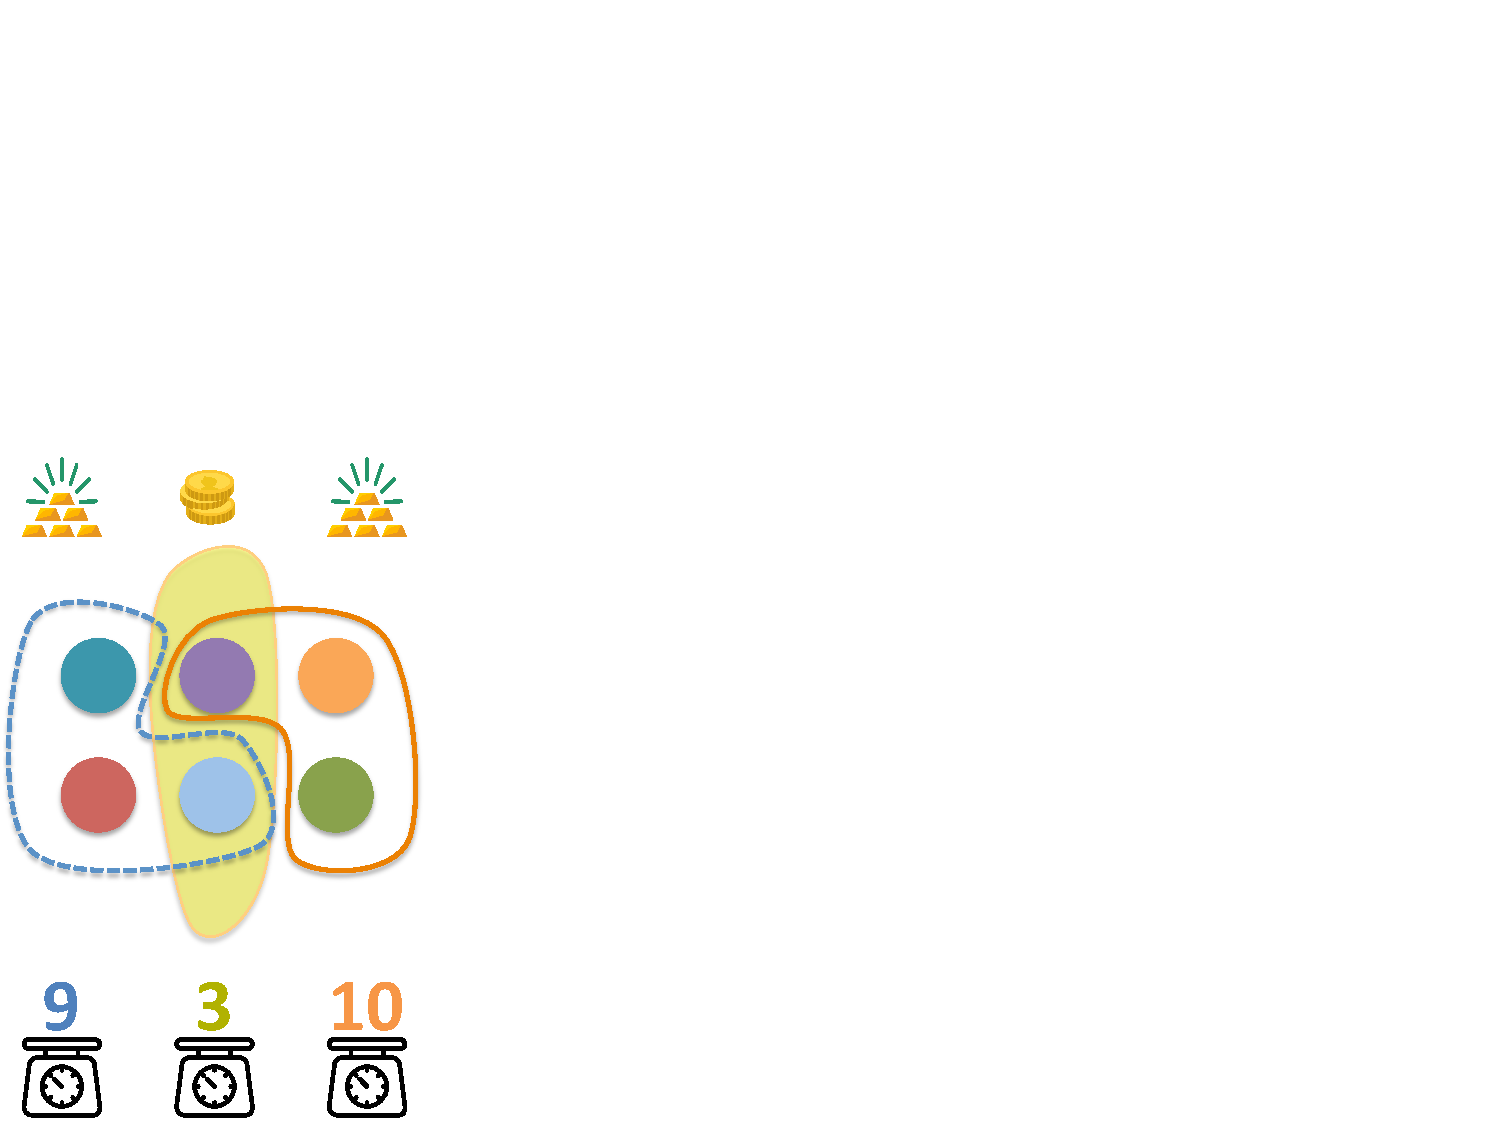
\includegraphics[width=\columnwidth]{value.pdf}\vfill}% 
\end{overlayarea}%
\end{minipage}%
\begin{minipage}{0.70\textwidth} 
\begin{itemize}
\item<1-> New Greedy Choice 
$$ best\_set = \arg \min_{j} \cfrac{w_j}{v_j} = \arg \min_{j} \cfrac{w_j}{\sum \text{value}(e_i)} $$
\item<2> Regular Greedy is a Special Case
 $$ \text{if value}(e_i) = 1 \rightarrow \cfrac{w_j}{\sum\text{value}(e_i)} = \cfrac{w_j}{|\hat{S}_j|}$$
\end{itemize}
\end{minipage}
\end{frame}

\begin{frame}
\frametitle{Another Heuristic Value Function..}
Dig Deeper, Extract more Information \inlinegraphics{excavators.eps}
\begin{minipage}{0.25\textwidth}
\only<1>{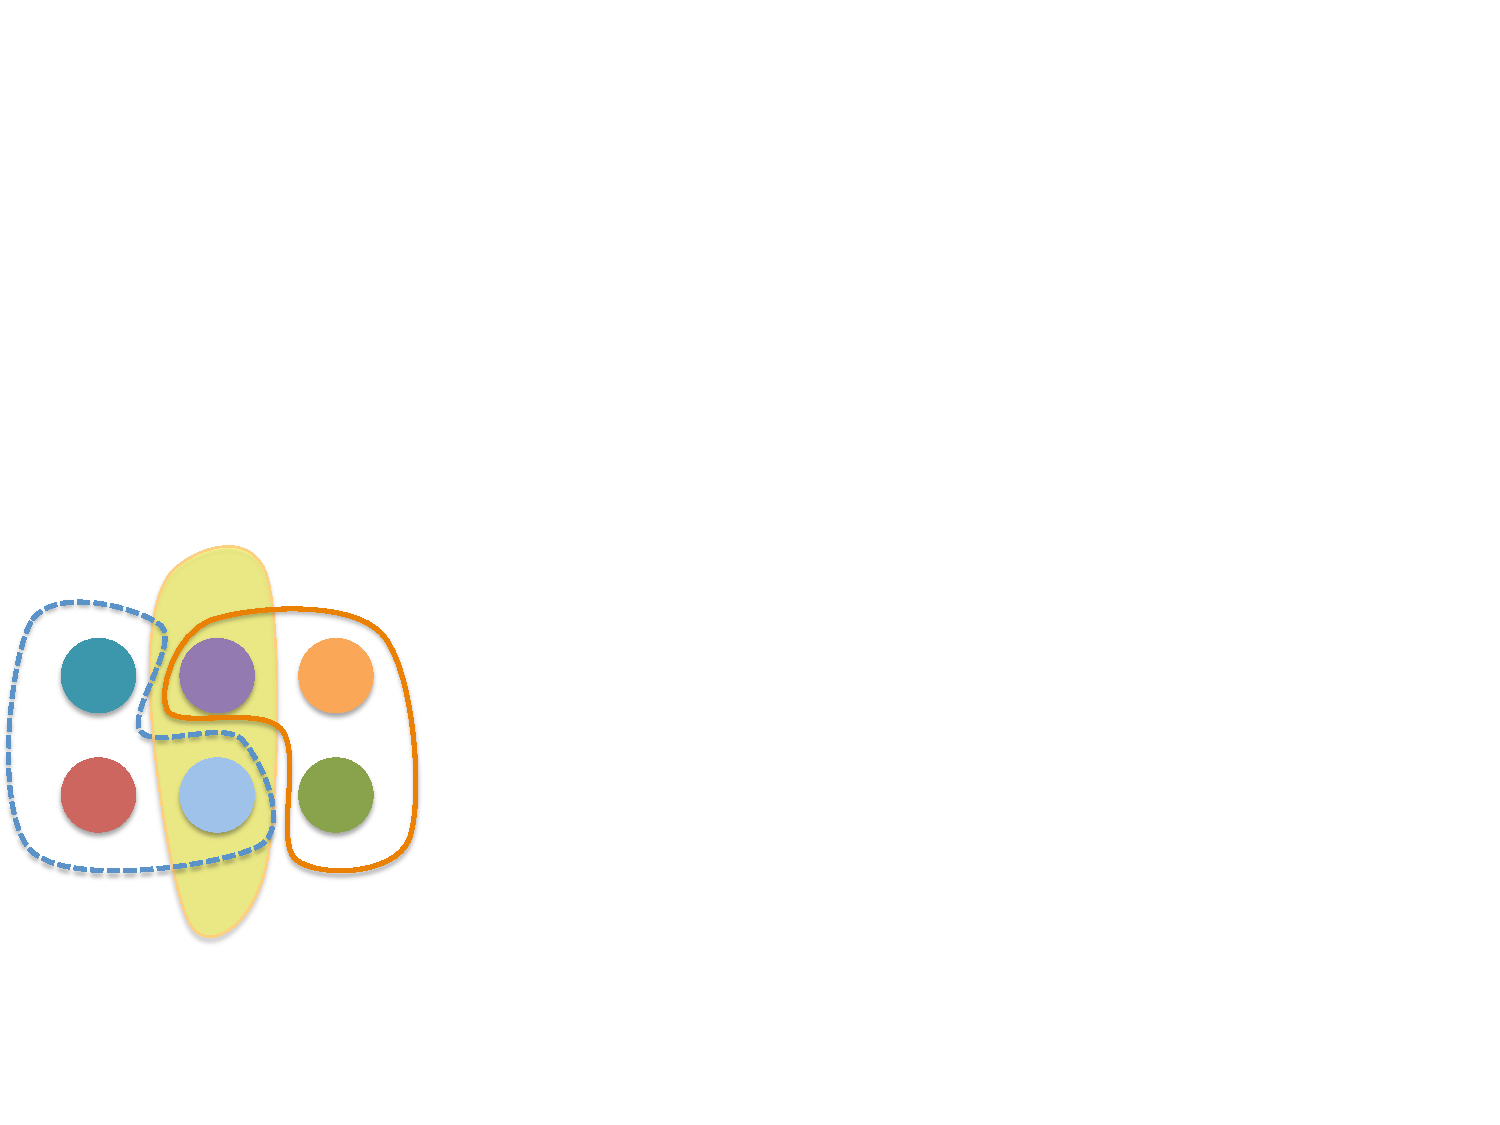
\includegraphics[width=\columnwidth]{frame2.pdf}}%
\end{minipage}%
\begin{minipage}{0.75\textwidth}
$$ \text{value}(e_i) = \cfrac{\sum_{S_j: e_i \in S_j} \text{average\_weight}(S_j)}{\text{frequency}(e_i)-1}$$
\end{minipage}
[\textbf{Intuition}]
\begin{itemize}
\item An element is valuable if it is contained in ``expensive'' sets.
\item Choose a ``\textbf{cheap}'' set that contains elements that are ``\textbf{expensive in the market}''.
\end{itemize}
\end{frame}

\begin{frame}
\frametitle{Theoretical Analysis}
\begin{block}{Approximation result}
Any greedy heuristic, caracterized by its value() function, is a $\displaystyle\frac{\displaystyle\max_{e_i} value(e_i)}{\displaystyle\min_{e_i} value(e_i)} \cdot H_n$-approximation.
\end{block}
\textbf{Remark:} This shows any greedy heuristics will have worse theoretical guarantees if our analysis is tight.
\end{frame}

\section{Experiments \& Results}
\begin{frame}
\frametitle{Value Functions Tested}
\begin{minipage}{0.50\textwidth}
\begin{itemize}
\item Greedy: $v(e_i) = 1$
\item H 1: $v(e_i) = \cfrac{1}{f_i -1}$
\item H 2: $v(e_i) = 1+\cfrac{1}{f_i -1}$
\item H 3: $v(e_i) = exp(-f_i)$
\item H 4: $v(e_i) = \cfrac{|\hat{S}_j|}{f_i -1}$
\item H 7: $v(e_i) = \cfrac{1}{(f_i -1)^2}$
\end{itemize}
\end{minipage}%
\begin{minipage}{0.50\textwidth}
\begin{itemize}
\item H 8: $v(e_i) = \cfrac{1}{(f_i -1)^3}$
\item H 9: $v(e_i) = \cfrac{1}{\sqrt{f_i -1}}$
\item H 10: $v(e_i) = \cfrac{\sum w_j/|\hat{S}_j|}{f_i -1}$
\item H 11: $v(e_i) = c + \cfrac{\sum w_j/|\hat{S}_j|}{f_i -1}$
\end{itemize}
\end{minipage}
\end{frame}

\begin{frame}
\frametitle{Data Sets}
\end{frame}

\begin{frame}
\frametitle{Experimental Results}

\adjustbox{max height=\dimexpr\textheight-5.5cm\relax,
           max width=\textwidth}{
  \begin{tabular}{*{8}{l}}
    \hline
    Heuristics & $\cfrac{1}{f_i -1} $& $1+\cfrac{1}{f_i -1}$& $ \cfrac{1}{(f_i -1)^2}$ & $\cfrac{1}{(f_i -1)^3}$ 
    & $\cfrac{1}{\sqrt{f_i -1}}$ & valuation-mixed & Greedy  \\
          \hline 
      Dataset 1 & 477 & \textcolor{LimeGreen}{461}&  477&  477&  \textcolor{LimeGreen}{461} & \textcolor{ProcessBlue}{463} & 463 \\
 Dataset 2 & \textcolor{LimeGreen}{566} & \textcolor{ProcessBlue}{572} & \textcolor{ProcessBlue}{580} & 588&  \textcolor{ProcessBlue}{572}&  \textcolor{ProcessBlue}{580} &  582 \\
 Dataset 3 &\textcolor{ProcessBlue}{564} & \textcolor{ProcessBlue}{589} & \textcolor{ProcessBlue}{552}&  \textcolor{LimeGreen}{547}&  \textcolor{ProcessBlue}{582}&  \textcolor{ProcessBlue}{596} & 598 \\
 Dataset 4 &\textcolor{LimeGreen}{540} & \textcolor{ProcessBlue}{541}&  561 & 550&  \textcolor{ProcessBlue}{541}&  \textcolor{ProcessBlue}{547} & 548 \\
 Dataset 5 &\textcolor{ProcessBlue}{575}&  \textcolor{ProcessBlue}{577}&  \textcolor{ProcessBlue}{573}&  \textcolor{LimeGreen}{567} & 584 & \textcolor{ProcessBlue}{577}&  577 \\
 Dataset 6 &\textcolor{ProcessBlue}{596} &  \textcolor{ProcessBlue}{606}& \textcolor{LimeGreen}{ 580}&  \textcolor{ProcessBlue}{588}&  \textcolor{ProcessBlue}{606}&  \textcolor{ProcessBlue}{606} & 615 \\
 Dataset 7 &480 & \textcolor{ProcessBlue}{474}&  \textcolor{LimeGreen}{461}&  \textcolor{ProcessBlue}{466} & 481&  \textcolor{ProcessBlue}{476} & 476 \\
 Dataset 8 &542 & \textcolor{LimeGreen}{533}&  542 & 548&  538 &  537 &  533\\
 Dataset 9 &\textcolor{ProcessBlue}{747} &  \textcolor{ProcessBlue}{744} &  \textcolor{ProcessBlue}{732} &  \textcolor{LimeGreen}{722}  & \textcolor{ProcessBlue}{746} &  \textcolor{ProcessBlue}{747}  & 747 \\
 Dataset 10 &290  & 291  & 291  & 290 &  291 &  292 &  289 \\
 Dataset 11 &\textcolor{ProcessBlue}{345} &  \textcolor{ProcessBlue}{343}  & \textcolor{LimeGreen}{339} &  \textcolor{ProcessBlue}{341}  & \textcolor{ProcessBlue}{343} &  \textcolor{ProcessBlue}{342}  & 348 \\
 Dataset 12 &\textcolor{ProcessBlue}{246}  & \textcolor{ProcessBlue}{246}  & \textcolor{LimeGreen}{245} &  252  & \textcolor{ProcessBlue}{246}  & \textcolor{ProcessBlue}{246}  & 246 \\
 Dataset 13 &\textcolor{ProcessBlue}{262} &  266 &  \textcolor{ProcessBlue}{265}  & \textcolor{LimeGreen}{257}  & 266  & 267 &  265 \\
 Dataset 14 &\textcolor{ProcessBlue}{234}  & \textcolor{ProcessBlue}{234}  & \textcolor{ProcessBlue}{235} &  \textcolor{ProcessBlue}{235}  & \textcolor{ProcessBlue}{234} &  \textcolor{LimeGreen}{233}  & 236 \\
Dataset 15 & \textcolor{ProcessBlue}{250}  & \textcolor{ProcessBlue}{250}  & \textcolor{ProcessBlue}{244}  & \textcolor{LimeGreen}{242}  & \textcolor{ProcessBlue}{250} &  \textcolor{ProcessBlue}{245} &  251 \\
 Dataset 16 & \textcolor{ProcessBlue}{317}  & \textcolor{ProcessBlue}{315}  & \textcolor{ProcessBlue}{311}  & \textcolor{LimeGreen}{310}  & \textcolor{ProcessBlue}{315}  & \textcolor{ProcessBlue}{320}  & 326 \\
 Dataset 17 & \textcolor{LimeGreen}{313}  & \textcolor{LimeGreen}{313} &  \textcolor{ProcessBlue}{314}  & \textcolor{ProcessBlue}{317} &  \textcolor{LimeGreen}{313}  & \textcolor{LimeGreen}{313}  & 323 \\
 Dataset 18 & \textcolor{LimeGreen}{304}  & \textcolor{ProcessBlue}{308} &  \textcolor{ProcessBlue}{307}  & 316 &  \textcolor{ProcessBlue}{308}  & \textcolor{LimeGreen}{304} &  312\\
 Dataset 19 & \textcolor{ProcessBlue}{159} &  160 &  164  & 163  & \textcolor{ProcessBlue}{159} &  \textcolor{LimeGreen}{157}  & 159 \\
 Dataset 20 & 171  & \textcolor{LimeGreen}{170} &  172  & 176  & 171  & \textcolor{LimeGreen}{170}  & 170 \\
 Dataset 21& \textcolor{ProcessBlue}{161}  & \textcolor{LimeGreen}{156}  & \textcolor{ProcessBlue}{159}  & \textcolor{ProcessBlue}{159} &  163  & \textcolor{LimeGreen}{156}  & 161 \\
 Dataset 22& \textcolor{ProcessBlue}{149}  & \textcolor{ProcessBlue}{149} &  \textcolor{ProcessBlue}{149}  & \textcolor{ProcessBlue}{148}  & \textcolor{ProcessBlue}{149}  & \textcolor{LimeGreen}{145} &  149 \\
 Dataset 23& \textcolor{ProcessBlue}{195} &  \textcolor{LimeGreen}{191}  & \textcolor{ProcessBlue}{194} &  203 &  \textcolor{ProcessBlue}{195} &  \textcolor{ProcessBlue}{192} &  196 \\
 Dataset 24 & \textcolor{LimeGreen}{545}  &  \textcolor{ProcessBlue}{548} &  565  & \textcolor{ProcessBlue}{554} &  557  & \textcolor{ProcessBlue}{550}  & 556 \\
     \hline
  \end{tabular}} 
   \begin{itemize}
\item<2-> Most of our heuristics are better than Greedy most of the time
\item<3-> The best heuristic varies a lot across datasets
\end{itemize}
\end{frame}


\begin{frame}
\frametitle{Experimental Results}
Here are the gains in percents of the greedy objective, for the top 6 heuristics:
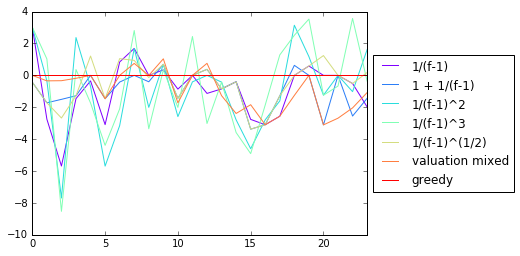
\includegraphics[width=\textwidth]{../results/heuristics_best6} \\
The best algorithm achieves a gain of \textbf{-0.96 \%}. If we combine all the algorithms, we have an average gain of \textbf{-2.88 \%}.
\end{frame}

\begin{frame}
\frametitle{References}
\begin{thebibliography}{1}
\bibitem{David} David Kordalewski, New Greedy Heuristics For Set Cover and Set Packing,CoRR, abs/1305.3584,2013.
\end{thebibliography}
\end{frame}

\end{document}
